\documentclass[compress]{beamer}

\usetheme{Berkeley}
\useoutertheme{smoothbars}
\useinnertheme{inmargin}
\usecolortheme{crane}
\usefonttheme{structurebold}
\usepackage{graphicx}

\begin{document}

\title{Military history of China before 1911}
\author{Zhang Yihan}
\institute{NEU ISE CS 1202}
\date{}

\begin{frame}
\titlepage
\end{frame}

\begin{frame}
\frametitle{Outline}
\tableofcontents
\end{frame}

\begin{frame}
\section{Summary}
The recorded military history of China extends from about 2200 BC to the present day. Although traditional Chinese Confucian philosophy favoured peaceful political solutions and showed contempt for brute military force, the military was influential in most Chinese states. Chinese pioneered the use of crossbows, advanced metallurgical standardization for arms and armour, early gunpowder weapons, and other advanced weapons, but also adopted nomadic cavalry and Western military technology. In addition, China's armies also benefited from an advanced logistics system as well as a rich strategic tradition, beginning with Sun Tzu's The Art of War, that deeply influenced military thought.
\end{frame}

\begin{frame}
\section{History of military organization}
\subsection{Pre-Warring States}
During the Shang and Western Zhou times, warfare was seen as an aristocratic affair, complete with protocols that may be compared to the chivalry of the European knight. States would not attack other states while mourning its ruler. Ruling houses would not be completely exterminated so descendants would be left to honor their ancestors.
\end{frame}

\begin{frame}
\begin{center}
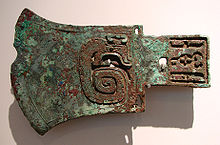
\includegraphics[width = 0.80\textwidth]{military-en/a.jpg} \\
A decorative bronze ax-head, dated 13th to 11th century BC, Shang Dynasty
\end{center}
\end{frame}

\begin{frame}
\subsection{Warring States}
By the time of the Warring States, reforms began that abolished feudalism and created powerful, centralized states. The power of the aristocracy was curbed and for the first time, professional generals were appointed on merit, rather than birth. Technological advances such as iron weapons and crossbows put the chariot-riding nobility out of business and favored large, professional standing armies, who were well-supplied and could fight a sustained campaign. The size of armies increased; whereas before 500 BC Chinese field armies numbered in the tens of thousands, by 300 BC armies regularly included up to a couple of hundred thousand drafted cowboys, accompanied by cavalry. For example, during the Battle of Changping the state of Qin drafted all males over 15 years of age.
\end{frame}

\begin{frame}
\begin{center}
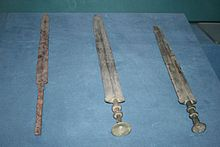
\includegraphics[width = 0.80\textwidth]{military-en/b.JPG} \\
An iron sword and two bronze swords from the Warring States period (403-221 BC)
\end{center}
\end{frame}

\begin{frame}
\subsection{Qin-Han}
Armies during the Qin and Han dynasties largely inherited their institutions from the earlier Warring States Period, with the major exception that cavalry forces were becoming more and more important, due to the threat of the Xiongnu. Under Emperor Wu of Han, the Chinese launched a series of massive cavalry expeditions against the Xiongnu, defeating them and conquering much of what is now Northern China, Western China, Mongolia, Central Asia, and Korea. After these victories, Chinese armies were tasked with the goal of holding the new territories against incursions and revolts by peoples such as the Qiang, Xianbei and Xiongnu who had come under Chinese rule.
\end{frame}

\begin{frame}
\begin{center}
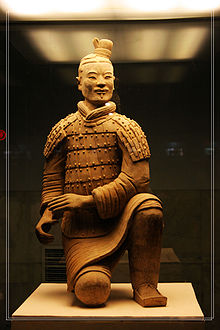
\includegraphics[width = 0.40\textwidth]{military-en/d.jpg} \\
Ceramic statues of infantry and cavalry, from the Han Dynasty (202 BC - 220 AD)
\end{center}
\end{frame}

\begin{frame}
\subsection{Era of division}
In 304 AD, a major event shook China. The Jin Dynasty, who had unified China 24 years earlier, was tottering in collapse due to a major civil war. Seizing this opportunity, Xiong-nu chieftain Liu Yuan and his forces revolted against their Han Chinese overlords. He was followed by many other barbarian leaders, and these rebels were called the "Wu Hu" or literally "Five barbarian tribes". By 316 AD, the Jin had lost all territory north of the Huai river. From this point on, much of North China was ruled by Sinicized barbarian tribes such as the Xianbei, while southern China remained under Han Chinese rule, a period known as the Era of Division. During this era, the military forces of both Northern and southern regimes diverged and developed very differently.
\end{frame}

\begin{frame}
\begin{center}
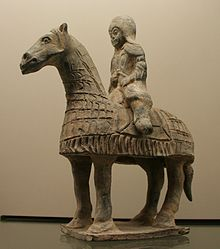
\includegraphics[width = 0.50\textwidth]{military-en/f.jpg} \\
A Chinese terracotta figurine of a cataphract horse and rider, created during the Northern Wei Dynasty (386 to 534 AD).
\end{center}
\end{frame}

\begin{frame}
\subsection{Northern}
Northern China was devastated by the Wu Hu uprisings. After the initial uprising, the various tribes fought among themselves in a chaotic era known as the Sixteen Kingdoms. Although brief unifications of the North, such as Later Zhao and Former Qin, occurred, these were relatively short-lived. During this era, the Northern armies, were mainly based around nomadic cavalry, but also employed Chinese as foot soldiers and siege personnel. This military system was rather improvising and ineffective, and the states established by the Wu Hu were mostly destroyed by the Jin Dynasty or the Xianbei.
\end{frame}

\begin{frame}
\begin{center}
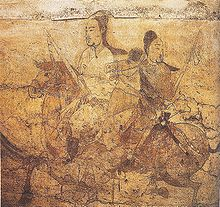
\includegraphics[width = 0.50\textwidth]{military-en/g.jpg} \\
Armed riders on horseback, a tomb mural from the Northern Qi (550-557 AD) period
\end{center}
\end{frame}

\begin{frame}
\subsection{Sui-Tang}
During the Sui and Tang, Chinese armies, based on the Fubing system invented during the era of division, won military successes that restored the empire of the Han Dynasty and reasserted Chinese power.[26] The Tang created large contingents of powerful heavy infantry. A key component of the success of Sui and Tang armies, just like the earlier Qin and Han armies, was the adoption of large elements of cavalry. These powerful horsemen, combined with the superior firepower of the Chinese infantry (powerful missile weapons such as recurve crossbows), made Chinese armies powerful.
\end{frame}

\begin{frame}
\begin{center}
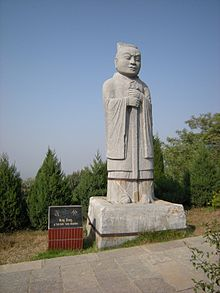
\includegraphics[width = 0.40\textwidth]{military-en/h.JPG} \\
A stone tomb guardian holding a sword, from the Tang Dynasty tombs at the Qianling Mausoleum
\end{center}
\end{frame}

\begin{frame}
\subsection{Yuan}
Founded by the Mongols who conquered Song China, the Yuan had the same military system as most nomadic peoples to China's north, focused mainly on nomadic cavalry, who were organized based on households and who were led by leaders appointed by the khan.
\end{frame}

\begin{frame}
\begin{center}
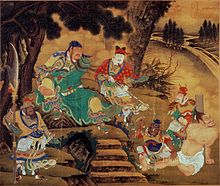
\includegraphics[width = 0.60\textwidth]{military-en/i.JPG} \\
"Guan Yu Captures General Pang De", a Ming Dynasty painting by Shang Xi
\end{center}
\end{frame}

\begin{frame}
\subsection{Qing}
The Qing dynasty engaged a western power for the second time in Chinese history, during the Russian–Manchu border conflicts, again defeating them in battle. The frontier in the south-west was extended slowly, in 1701 the Qing defeated the Tibetans at the Battle of Dartsedo. The Manchus extended their power to the west, conquering modern Xinjiang and establishing a protectorate over Tibet. After the demise of the Zunghar Khanate, Manchu authority in Tibet faced only weak opposition. In 1792-1793 the Qing carried out the military campaign to drive the Gurkhas out of Tibet and only stopped their chase near Kathmandu. In 1841 the Sino-Sikh war ended with the expulsion of a Sikh army.
\end{frame}

\begin{frame}
\begin{center}
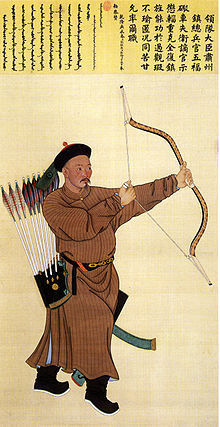
\includegraphics[width = 0.30\textwidth]{military-en/j.jpg} \\
Portrait of Wu Fu, Brigadier General of the Gansu Region. Hanging scroll; ink and color on silk; 1760 AD; inscribed, and with one seal of the Qianlong Emperor.
\end{center}
\end{frame}

\begin{frame}
\section{Modernization}
\begin{center}
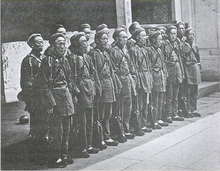
\includegraphics[width = 0.80\textwidth]{military-en/k.png} \\
Chinese Troops trained by foreigners 1867-1868
\end{center}
\end{frame}

\begin{frame}
\begin{center}
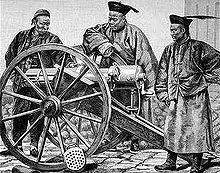
\includegraphics[width = 0.80\textwidth]{military-en/l.jpg} \\
Chinese Qing Empire officers with the French Montigny mitrailleuse gun.
\end{center}
\end{frame}

\begin{frame}
\begin{center}

\includegraphics[width = \textwidth]{AwwYeah.jpg} \\
Thank you!
\end{center}
\end{frame}

\end{document}
